% Options for packages loaded elsewhere
% Options for packages loaded elsewhere
\PassOptionsToPackage{unicode}{hyperref}
\PassOptionsToPackage{hyphens}{url}
\PassOptionsToPackage{dvipsnames,svgnames,x11names}{xcolor}
%
\documentclass[
  11pt,
]{article}
\usepackage{xcolor}
\usepackage[margin = 1in]{geometry}
\usepackage{amsmath,amssymb}
\setcounter{secnumdepth}{-\maxdimen} % remove section numbering
\usepackage{iftex}
\ifPDFTeX
  \usepackage[T1]{fontenc}
  \usepackage[utf8]{inputenc}
  \usepackage{textcomp} % provide euro and other symbols
\else % if luatex or xetex
  \usepackage{unicode-math} % this also loads fontspec
  \defaultfontfeatures{Scale=MatchLowercase}
  \defaultfontfeatures[\rmfamily]{Ligatures=TeX,Scale=1}
\fi
\usepackage{lmodern}
\ifPDFTeX\else
  % xetex/luatex font selection
  \setmainfont[]{Palatino}
  \setmathfont[]{STIX Two Math}
\fi
% Use upquote if available, for straight quotes in verbatim environments
\IfFileExists{upquote.sty}{\usepackage{upquote}}{}
\IfFileExists{microtype.sty}{% use microtype if available
  \usepackage[]{microtype}
  \UseMicrotypeSet[protrusion]{basicmath} % disable protrusion for tt fonts
}{}
\usepackage{setspace}
\makeatletter
\@ifundefined{KOMAClassName}{% if non-KOMA class
  \IfFileExists{parskip.sty}{%
    \usepackage{parskip}
  }{% else
    \setlength{\parindent}{0pt}
    \setlength{\parskip}{6pt plus 2pt minus 1pt}}
}{% if KOMA class
  \KOMAoptions{parskip=half}}
\makeatother


\usepackage{longtable,booktabs,array}
\usepackage{calc} % for calculating minipage widths
% Correct order of tables after \paragraph or \subparagraph
\usepackage{etoolbox}
\makeatletter
\patchcmd\longtable{\par}{\if@noskipsec\mbox{}\fi\par}{}{}
\makeatother
% Allow footnotes in longtable head/foot
\IfFileExists{footnotehyper.sty}{\usepackage{footnotehyper}}{\usepackage{footnote}}
\makesavenoteenv{longtable}
\usepackage{graphicx}
\makeatletter
\newsavebox\pandoc@box
\newcommand*\pandocbounded[1]{% scales image to fit in text height/width
  \sbox\pandoc@box{#1}%
  \Gscale@div\@tempa{\textheight}{\dimexpr\ht\pandoc@box+\dp\pandoc@box\relax}%
  \Gscale@div\@tempb{\linewidth}{\wd\pandoc@box}%
  \ifdim\@tempb\p@<\@tempa\p@\let\@tempa\@tempb\fi% select the smaller of both
  \ifdim\@tempa\p@<\p@\scalebox{\@tempa}{\usebox\pandoc@box}%
  \else\usebox{\pandoc@box}%
  \fi%
}
% Set default figure placement to htbp
\def\fps@figure{htbp}
\makeatother





\setlength{\emergencystretch}{3em} % prevent overfull lines

\providecommand{\tightlist}{%
  \setlength{\itemsep}{0pt}\setlength{\parskip}{0pt}}



 


%%% Setup for frontmatter, spacing, and colors %%%

\usepackage{orcidlink} % for Orchid ID

% set the geometry of the document
\usepackage{indentfirst} % indent first para
\setlength{\parindent}{0.5in} % set indent length
\setlength{\parskip}{0em} % no extra space between paras

% set spacing of section titles
\usepackage{titlesec} % to set spacing of section titles
\titlespacing\section{0pt}{0pt plus 2pt minus 2pt}{0pt plus 2pt minus 2pt}
\titlespacing\subsection{0pt}{0pt plus 2pt minus 2pt}{0pt plus 2pt minus 2pt}
\titlespacing\subsubsection{0pt}{0pt plus 2pt minus 2pt}{0pt plus 2pt minus 2pt}

%%% Figures and Tables %%%

% captions 
\usepackage{caption}
\captionsetup{
  %captionskip = 0pt,   % eliminate space bw capiton and figure
  %font = bf,            % make the font of the entire caption bold
  %font = footnotesize,         % make font of entire caption smaller
  justification = raggedright, % left justify the caption 
  singlelinecheck = true,      % but only if it is more than one line
  labelfont = bf               % make the caption label bold
}
\setlength{\abovecaptionskip}{10pt} % Adjust the space above the caption

% for rotating figures and tables
\usepackage{rotating}        
\usepackage{pdflscape}

%%% Abstract %%%

\usepackage{abstract}
\renewcommand{\abstractname}{ABSTRACT\vspace{.5em}}
\renewcommand{\abstractnamefont}{\normalfont\bfseries}
\renewcommand{\abstracttextfont}{\normalsize}
\setlength{\absleftindent}{\parindent}
\setlength{\absrightindent}{\parindent}

%% Title %%%

\usepackage{titling}
%\setlength{\droptitle}{3em}
\pretitle{\par\vskip 3em\begin{center}\LARGE\bfseries}
\posttitle{\par\end{center}\vspace{2\baselineskip}}

%%% New commands %%%

% Keywords
\providecommand{\keywords}[1]{\textbf{\textit{Keywords---}}#1}

% Keywords
\providecommand{\fundinginfo}[1]{\textbf{\textit{Funding: }}#1}

% Word count
\providecommand{\wordcount}[1]{\textbf{Word Count: }#1}

% Conflicts
\providecommand{\conflicts}[1]{\textbf{\textit{Conflicts of Interest: }}#1}

% Command for a note at the top of the first page describing the publication
% status of the paper.
\newcommand{\published}[1]{%
   \gdef\puB{#1}}
   \newcommand{\puB}{}
   \renewcommand{\maketitlehooka}{%
       \par\noindent\footnotesize\sffamily\puB}
\usepackage{booktabs}
\usepackage{caption}
\usepackage{longtable}
\usepackage{colortbl}
\usepackage{array}
\usepackage{anyfontsize}
\usepackage{multirow}
\makeatletter
\@ifpackageloaded{caption}{}{\usepackage{caption}}
\AtBeginDocument{%
\ifdefined\contentsname
  \renewcommand*\contentsname{Table of contents}
\else
  \newcommand\contentsname{Table of contents}
\fi
\ifdefined\listfigurename
  \renewcommand*\listfigurename{List of Figures}
\else
  \newcommand\listfigurename{List of Figures}
\fi
\ifdefined\listtablename
  \renewcommand*\listtablename{List of Tables}
\else
  \newcommand\listtablename{List of Tables}
\fi
\ifdefined\figurename
  \renewcommand*\figurename{Figure}
\else
  \newcommand\figurename{Figure}
\fi
\ifdefined\tablename
  \renewcommand*\tablename{Table}
\else
  \newcommand\tablename{Table}
\fi
}
\@ifpackageloaded{float}{}{\usepackage{float}}
\floatstyle{ruled}
\@ifundefined{c@chapter}{\newfloat{codelisting}{h}{lop}}{\newfloat{codelisting}{h}{lop}[chapter]}
\floatname{codelisting}{Listing}
\newcommand*\listoflistings{\listof{codelisting}{List of Listings}}
\makeatother
\makeatletter
\makeatother
\makeatletter
\@ifpackageloaded{caption}{}{\usepackage{caption}}
\@ifpackageloaded{subcaption}{}{\usepackage{subcaption}}
\makeatother
\usepackage{bookmark}
\IfFileExists{xurl.sty}{\usepackage{xurl}}{} % add URL line breaks if available
\urlstyle{same}
\hypersetup{
  pdftitle={Extracting Event Counts and Locations from Conflict Reports},
  pdfauthor={Emmanuel Teitelbaum},
  colorlinks=true,
  linkcolor={Blue4},
  filecolor={Maroon},
  citecolor={Blue4},
  urlcolor={Blue4},
  pdfcreator={LaTeX via pandoc}}


%% Main title %%

\title{Extracting Event Counts and Locations from Conflict
Reports\thanks{I am grateful to Mohiddin Bacha Shaik and Shiva Sharma
for their excellent research assitance.}}

%% Subtitle %%

\usepackage{etoolbox}
\makeatletter
\providecommand{\subtitle}[1]{% add subtitle to \maketitle
  \apptocmd{\@title}{\par {\vskip 0.25em \large #1 \par}}{}{}
}
\makeatother
\subtitle{Evidence from the South Asia Terrorism Portal}

%% Author info %%

  \author{Emmanuel Teitelbaum\thanks{Corresponding author.}
~\orcidlink{0000-0001-7089-0588}
\\George Washington University
\\Department of Political Science
\\\href{mailto:ejt@gwu.edu}{ejt@gwu.edu}
 }

% Omit the date since the \published command does that
\date{}  % blank date

\usepackage{url}
\urlstyle{same}
\begin{document}
%%% Title Section %%%

\newgeometry{top=0.5in, bottom=1in, left=1in, right=1in}

\published{\textbf{2026-04-08} \qquad Prepared for the APSA Virtual
Research Meeting. \\ {\scriptsize Access the code, data, and analysis at
\url{https://github.com/eteitelbaum/code-satp.git}}}

\vspace{0.25in}

\maketitle

\vspace{0.25in}

%%% Abstract %%%


\vspace{0.25in}

%%% Word Count %%%


\vspace{0.25in}

%%% Funding %%%

\noindent
\fundinginfo{This project received funding from the Smith Richardson
Foundation and in-kind support from the GW Institute for International
Economic Policy.}

%%% Conflicts %%%


\restoregeometry

\setstretch{1.5}
\section{Introduction}\label{introduction}

{[}Introduction text to be written.{]}

\section{Data and Methods}\label{data-and-methods}

{[}Methods text to be written.{]}

\section{Results}\label{results}

\subsection{Baseline Model
Comparisons}\label{baseline-model-comparisons}

{[}Results text to be written. Tables Table~\ref{tbl-seq2seq-baseline}
and Table~\ref{tbl-llm-baseline} report overall performance for the
seq2seq and LLM model families respectively. Values in bold are
significantly better than the ConfliBERT-Poisson baseline (paired
bootstrap, \(n = 5{,}000\) replications, \(p < .05\)); a dagger (†)
indicates the model is not significantly different from the ceiling
model.{]}

\begin{table}

\caption{\label{tbl-seq2seq-baseline}Death count extraction performance:
seq2seq models.}

\centering{

\fontsize{8.0pt}{9.0pt}\selectfont
\begin{tabular*}{\linewidth}{@{\extracolsep{\fill}}lrllrrlr}
\toprule
Metric & {\bfseries ConfliBERT} & T5-Base & T5-Large & IndicBART & mT5-Base & NT5-Small & {\bfseries T5-XL} \\ 
\midrule\addlinespace[2.5pt]
MAE & 0.37 & 0.27 & {\bfseries 0.16†} & 0.33 & 0.27 & 0.29 & {\bfseries 0.12} \\ 
RMSE & 2.21 & 3.21 & 1.18† & 1.73 & 1.61 & 3.11 & {\bfseries 0.85} \\ 
Within-1 & 94.6 & {\bfseries 97.7†} & {\bfseries 97.8†} & 94.9 & {\bfseries 96.3} & {\bfseries 97.3†} & {\bfseries 98.1} \\ 
Within-2 & 97.3 & {\bfseries 98.6†} & {\bfseries 98.7†} & 96.5 & 97.7 & {\bfseries 98.4†} & {\bfseries 98.7} \\ 
Nonzero MAE & 0.56 & 0.39 & {\bfseries 0.21†} & 0.42 & {\bfseries 0.30} & {\bfseries 0.39} & {\bfseries 0.15} \\ 
\bottomrule
\end{tabular*}
\begin{minipage}{\linewidth}
\vspace{.05em}
Bold = significantly better than ConfliBERT (paired bootstrap, n = 5000, p < .05). † = not significantly different from ceiling (p > .05). MAE and Nonzero MAE: lower is better. Within-1 and Within-2: higher is better.\\
\end{minipage}

}

\end{table}%

\begin{table}

\caption{\label{tbl-llm-baseline}Death count extraction performance:
large language models.}

\centering{

\fontsize{8.0pt}{9.0pt}\selectfont
\begin{tabular*}{\linewidth}{@{\extracolsep{\fill}}lrlllr}
\toprule
Metric & {\bfseries ConfliBERT} & Llama-3.1-8B & Mistral-7B & Mixtral-8x7B & {\bfseries GPT-4o-mini} \\ 
\midrule\addlinespace[2.5pt]
MAE & 0.37 & 0.23† & 0.30 & 0.30† & {\bfseries 0.13} \\ 
RMSE & 2.21 & 2.77† & 3.04 & 3.75† & {\bfseries 0.94} \\ 
Within-1 & 94.6 & {\bfseries 97.7†} & {\bfseries 97.2†} & {\bfseries 97.9†} & {\bfseries 97.9} \\ 
Within-2 & 97.3 & 98.4† & 97.8 & {\bfseries 98.5†} & {\bfseries 98.6} \\ 
Nonzero MAE & 0.56 & {\bfseries 0.19†} & {\bfseries 0.22†} & {\bfseries 0.16†} & {\bfseries 0.17} \\ 
\bottomrule
\end{tabular*}
\begin{minipage}{\linewidth}
\vspace{.05em}
Bold = significantly better than ConfliBERT (paired bootstrap, n = 5000, p < .05). † = not significantly different from ceiling (p > .05). MAE and Nonzero MAE: lower is better. Within-1 and Within-2: higher is better.\\
\end{minipage}

}

\end{table}%

\subsection{Bin-Level Performance}\label{bin-level-performance}

\textbf{?@fig-heatmap-seq2seq}

\begin{figure}

\centering{

\pandocbounded{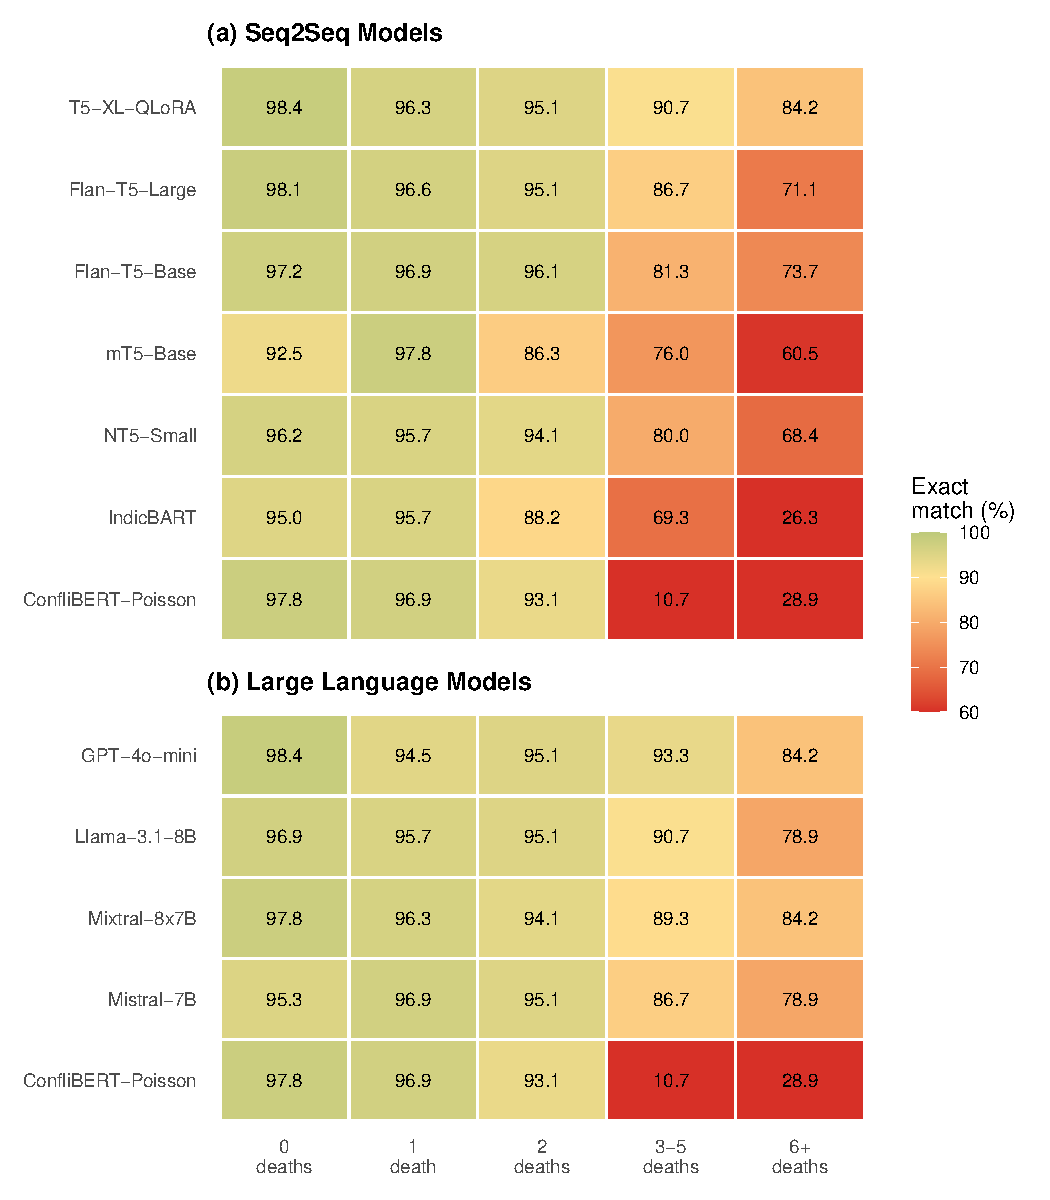
\includegraphics[keepaspectratio]{satp-counts_files/figure-pdf/fig-heatmap-combined-1.pdf}}

}

\caption{\label{fig-heatmap-combined}Exact match (\%) by death count
bin. Seq2seq models (top) and LLMs (bottom), each ordered by overall MAE
(best at top). ConfliBERT-Poisson appears in both panels as a reference
baseline.}

\end{figure}%

\subsection{Rare-Bin Improvement
Strategies}\label{rare-bin-improvement-strategies}

\subsubsection{Seq2Seq Training-Side
Interventions}\label{seq2seq-training-side-interventions}

Table~\ref{tbl-rarebin-seq2seq}

\begin{table}

\caption{\label{tbl-rarebin-seq2seq}Seq2seq rare-bin intervention
results (Flan-T5-Large base).}

\centering{

\fontsize{8.0pt}{9.0pt}\selectfont
\begin{tabular*}{\linewidth}{@{\extracolsep{\fill}}lllllllr}
\toprule
Metric & Baseline & Weighted & Loss Wt. & Targeted & Back-transl. & Paraphrase & {\bfseries T5-XL} \\ 
\midrule\addlinespace[2.5pt]
MAE & 0.16† & 0.26 & 0.22† & 0.24† & 0.27 & 0.27 & 0.12 \\ 
Nonzero MAE & 0.21† & 0.36 & 0.35 & 0.35 & 0.37 & 0.38 & 0.15 \\ 
Bin 3-5 MAE & 0.24† & 0.27 & 0.24 & 0.24 & 0.21† & 0.23† & 0.19 \\ 
Bin 3-5 Exact (\%) & 86.7† & 85.3 & 86.7† & 85.3 & 88.0† & 86.7† & 90.7 \\ 
Bin 6+ MAE & 1.97† & 4.08 & 3.95 & 4.05 & 4.18 & 4.34 & 1.05 \\ 
Bin 6+ Exact (\%) & 71.1† & 73.7† & 68.4 & 68.4 & 71.1 & 71.1 & 84.2 \\ 
\bottomrule
\end{tabular*}
\begin{minipage}{\linewidth}
\vspace{.05em}
Bold = significantly better than baseline model (paired bootstrap, n = 5000, p < .05). † = not significantly different from ceiling (p > .05). MAE rows: lower is better. Exact (\%) rows: higher is better.\\
\end{minipage}

}

\end{table}%

\subsubsection{LLM Prompt Engineering
Interventions}\label{llm-prompt-engineering-interventions}

Table~\ref{tbl-rarebin-llms}

\begin{table}

\caption{\label{tbl-rarebin-llms}LLM prompt engineering results
(Llama-3.1-8B base).}

\centering{

\fontsize{8.0pt}{9.0pt}\selectfont
\begin{tabular*}{\linewidth}{@{\extracolsep{\fill}}llllllr}
\toprule
Metric & Baseline & Protocol & Bin-shot & Hard-shot & Combined & {\bfseries GPT-4o-mini} \\ 
\midrule\addlinespace[2.5pt]
MAE & 0.23† & 0.32 & {\bfseries 0.20†} & {\bfseries 0.11†} & {\bfseries 0.11†} & 0.13 \\ 
Nonzero MAE & 0.19† & 0.20† & 0.15† & 0.14† & 0.13† & 0.17 \\ 
Bin 3-5 MAE & 0.20† & 0.23† & 0.28 & 0.20† & 0.28 & 0.16 \\ 
Bin 3-5 Exact (\%) & 90.7† & 88.0† & 88.0 & 90.7† & 88.0 & 93.3 \\ 
Bin 6+ MAE & 1.53† & 0.95† & 0.97† & 0.84† & {\bfseries 0.63†} & 1.24 \\ 
Bin 6+ Exact (\%) & 78.9† & 76.3† & 78.9† & 81.6† & {\bfseries 89.5†} & 84.2 \\ 
\bottomrule
\end{tabular*}
\begin{minipage}{\linewidth}
\vspace{.05em}
Bold = significantly better than baseline model (paired bootstrap, n = 5000, p < .05). † = not significantly different from ceiling (p > .05). MAE rows: lower is better. Exact (\%) rows: higher is better.\\
\end{minipage}

}

\end{table}%

\section{Discussion}\label{discussion}

{[}Discussion text to be written.{]}

\newpage

\section{Appendix}\label{appendix}

\newpage

\section{References}\label{references}

\setlength{\parindent}{-0.2in}
\setlength{\leftskip}{0.2in}
\setlength{\parskip}{8pt}
\noindent




\end{document}
